\documentclass[instructions]{./Packages/uqthesis}
% ***************************************************
% LaTeX Packages
% ***************************************************
% This file defines the document design.
% Usually it is not necessary to edit this file, but you can use it to change aspects of the design if you want.

%There are essential packages that are contained within the uqthesis.cls which are integral to the template - These must not be deleted.  A list of these packages can be found in the README.tet file

%The packages below are optional, please add or alter as required.

\usepackage{cite}				 %Allows abbreviated numerical citations.
\usepackage{pdfpages}			 %Allows you to include full-page pdfs.
\usepackage{wrapfig}			 %Lets you wrap text around figures.
\usepackage{bm} 				 %Bolded maths characters.
\usepackage{upgreek}			 %Upright Greek characters.
\usepackage{dsfont}				 %Double-struck fonts.
\usepackage{simplewick}			 %For typesetting Wick contractions.
\usepackage{mathtools}		     %Can be used to fine-tune the maths presentation.	
\usepackage{framed}			     %For boxed text.
\usepackage{microtype}			 %pdfLaTeX will fix your kerning.
\usepackage{marvosym}			 %Include symbols (like the Euro symbol, etc.).
\usepackage{color}				 %Nice for scalable pdf graphics using InkScape.
\usepackage{transparent}	     %Nice for scalable pdf graphics using InkScape.
\usepackage{placeins}			 %Lets you put in a \FloatBarrier to stop figures floating past this command.
\usepackage{mdframed,mdwlist}    %Use these for nice lists (less white space).
\usepackage{graphicx}            %Enhanced support for graphics.
\usepackage{float}               %Improved interface for floating objects. 
\usepackage{longtable}           %Allow tables to flow over page boundaries.
\usepackage{mathdots}            %Changed the basic LaTeX and plain TeX commands.
\usepackage{eucal}               %Font shape definitions to use the Euler script symbols in math mode.
\usepackage{array}               %Extending the array and tabular environments.
\usepackage{stmaryrd}            %The StMary’s Road symbol font.
\usepackage{amsthm}              %St Mary Road symbols for theoretical computer science. 
\usepackage{pifont}              %Access to PostScript standard Symbol and Dingbats fonts.
\usepackage{lipsum}              %Easy access to the Lorem Ipsum dummy text.
\usepackage{enumerate}           %Enumerate with redefinable labels. 
\usepackage[all]{xy}             %This is a special package for drawing diagrams.
\usepackage{amsmath}             %ATypesetting theorems (AMS style).
\usepackage{amssymb}             %Provided an extended symbol collection.
\usepackage[utf8]{inputenc}      %Allowed all displayable utf8 characters to be available as input.
\usepackage{fancyhdr}            %Extensive control of page headers and footers.
\usepackage{blindtext}           %Produced 'blind' text for testing.
\usepackage{tikz}                %To create graphic elements.
\usepackage[figuresright]{rotating}	%Allows large tables to be rotated to landscape.
\usetikzlibrary{shapes.geometric, arrows}
%You can add more packages here if you need


%This defines some macros that implement Latin abbreviations
%COMMENT OUT OR DELETE IF UNDESIRED.
\newcommand{\via}{\textit{via}} %Italicised via.
\newcommand{\ie}{\textit{i.e.}} %Literally.
\newcommand{\eg}{\textit{e.g.}} %For example.
\newcommand{\etc}{\textit{etc.}} %So on...
\newcommand{\vv}{\textit{vice versa}} %And the other way around.
\newcommand{\viz}{\textit{viz}.} %Resulting in.
\newcommand{\cf}{\textit{cf}.} %See, or 'consistent with'.
\newcommand{\apr}{\textit{a priori}} %Before the fact.
\newcommand{\apo}{\textit{a posteriori}} %After the fact.
\newcommand{\vivo}{\textit{in vivo}} %In the flesh.
\newcommand{\situ}{\textit{in situ}} %On location.
\newcommand{\silico}{\textit{in silico}} %Simulation.
\newcommand{\vitro}{\textit{in vitro}} %In glass.
\newcommand{\vs}{\textit{versus}} %James \vs{} Pete.
\newcommand{\ala}{\textit{\`{a} la}} %In the manner of...
\newcommand{\apriori}{\textit{a priori}} %Before hand.
\newcommand{\etal}{\textit{et al.}} %And others, with correct punctuation.
\newcommand{\naive}{na\"\i{}ve} %Queen Amidala is young and \naive{}.
\usepackage{listings}
\usepackage{xcolor} % for custom colors (optional)

\lstset{
  basicstyle=\ttfamily\small,        % typewriter font and smaller size
  numbers=left,                      % line numbers on the left
  numberstyle=\tiny\color{gray},     % style of line numbers
  stepnumber=1,                      % number every line
  numbersep=10pt,                    % distance between line numbers and code
  showstringspaces=false,           % don't show spaces in strings
  tabsize=2,                         % tab size
  breaklines=true,                  % wrap long lines
  frame=none,                     % put a frame around the code
  language=Java                     % or another language if appropriate
}
\footskip 30pt
\title{Prolog Optimizations in GraalVM}
\author{Thi Thuy Tien Nguyen}
\currentdegrees{Master of Computer Science (Management)}
\orcid{\href{add your ORCID url here}{Candidate's ORCID}}
\date{9 May 2025}
\school{School of Electrical Engineering and Computer Science}
\university{The University of Queensland}

\titleformat{\chapter}{\LARGE\bfseries}{\thechapter}{1em}{\LARGE}
\titlespacing{\chapter}{0pt}{-10pt}{5pt}
\titlespacing{\section}{0pt}{8pt}{5pt}
\titlespacing{\subsection}{0pt}{10pt}{5pt}
\begin{document}
\maketitle
\thispagestyle{empty}
\clearpage

\input{./Letter/Letter.tex}
\thispagestyle{empty}
\clearpage

\renewcommand{\sectionmark}[1]{\markboth{\thesection~#1}{}}

\frontmatter
\openany

\begin{KeepFromToc}
    \setcounter{page}{0} %reset the page counter
    \tableofcontents
    \newpage
    \listoffigures
    \newpage
    \listoftables
\end{KeepFromToc}
  \let\cleardoublepage\clearpage

\mainmatter

\chapter[Abstract]{Abstract}

\noindent
Compiler optimizations are critical for enhancing program execution speed and overall performance. This thesis proposes integrating Prolog-based optimization techniques into the GraalVM compiler framework to potentially enhance compiler performance. The approach involves developing a Prolog-based optimizer that translates GraalVM’s intermediate representation (IR) of programs into Prolog facts and defines optimization rules using Prolog’s declarative syntax. By querying these rules within the GraalVM compiler, the proposal aims to explore how Prolog’s logic programming capabilities can improve the expressiveness and effectiveness of compiler optimizations. The study seeks to assess the feasibility of this integration, examining how Prolog’s declarative nature might contribute to more sophisticated and potentially more efficient optimization strategies compared to traditional imperative methods. This approach could lead to advancements in compiler technology and open new avenues for research in the optimization phase of compilation. The project spans 30 weeks, divided into two semesters and four phases: Project Proposal, Proof of Concept, Extension and Evaluation, and Report and Demonstration, with 10 hours of work per week. The first semester focused on initial research and development of a proof of concept, and the second half on refining, expanding and preparing the final deliverables.
\chapter[Introduction]{Introduction}

Compiler optimizations seek to improve program execution speed and overall performance, which can result in substantial cost savings for large-scale organizations, potentially reducing infrastructure expenses by millions annually. This project aims to assess the feasibility of implementing an optimizer in logic programming language within the GraalVM compiler framework. Specifically, this project examines the integration of GraalVM Ahead-of-Time (AOT) compiler optimizations with Prolog. The project works with AOT due to its advantages over Just-In-Time (JIT) compilation, which involves runtime code compilation that incurs higher overhead in terms of CPU and memory usage and introduces delays through dynamic optimization and profiling. In contrast, AOT compilation completes all compilation and optimizations at build time with minimal runtime overhead. 

Logic programming languages with declarative specifications allow programs to be analyzed efficiently through queries, enabling the implementation of code optimization that would otherwise be difficult to achieve. By focusing on what needs to be achieved rather than how to achieve it, declarative approaches offer greater clarity and intuitiveness. This inherent simplicity and readability facilitate the experimentation and development of new optimization rules, as well as the maintenance of existing ones. Additionally, declarative code is easier to debug, test, and ensure correctness because it is more straightforward and easier to follow. Previous research has extensively utilized Datalog, a prominent logic programming language, for different levels of program analysis \cite{Bravenboer2009,Tonder2021,Lam2005,Benton2007}. However, there is a notable lack of prior work regarding the application of logic programming languages for the optimization and transformation of code. Spinellis’ work in 1999 explored an alternative method for expressing optimizations through declarative specifications, as opposed to traditional imperative code \cite{Spinellis1999}. However, Spinellis’s work was limited to a rudimentary prototype of an optimizer with a ``single optimization specification" and ``limited flow-of-control optimizations" \cite{Spinellis1999}.

The proposed approach involves three main steps. First, optimization rules are defined as Prolog facts and predicates, focusing on canonicalization to standardize the IR code and conditional elimination to remove redundant expressions. Second, the Prolog fact generator parses the IR and converts it into Prolog facts, ensuring compatibility with optimization rules for effective query-based optimization. Finally, the Prolog-based optimizer is developed in Java to recursively query these rules, apply transformations, and refine the IR iteratively. As each optimization is applied, the IR is updated and reconstructed based on the optimized Prolog facts, leading to an improved representation of the program. To ensure correctness, a comprehensive test suite will be created to verify Prolog rule functionality, validate generated facts, and ensure the correctness of the optimized code. The performance will be evaluated based on execution speed, resource usage, and optimization throughput, alongside an assessment of whether Prolog’s declarative syntax improves optimization expressibility, documentation, comprehension, and maintenance.

\chapter[Background and Related Works]{Background}

\section{Background Materials}
\subsection{Ahead-of-time (AOT) Compilation}
In the Java Virtual Machine (JVM), byte code compilation can occur either at build time or runtime. Ahead-of-Time (AOT) compilation involves translating the byte code into machine code before execution, resulting in a fully compiled binary that is immediately executable \cite{Wade2017}. In contrast, Just-In-Time (JIT) Compilation defers the translation until runtime if at all, dynamically converting Java bytecodes into machine code within the Java Virtual Machine (JVM) and optimizing frequently executed code paths to enhance performance \cite{Wade2017}. AOT compilation generally requires longer build times but offers rapid startup and predictable performance, making it suitable for applications where quick initialization is critical. JIT compilation, while benefiting from shorter build times, incurs longer startup periods but allows for more complex optimizations based on runtime profiling data.

JIT compilation enables techniques such as speculative optimizations, which make assumptions about a program’s behavior to apply performance-enhancing transformations based on runtime profiling. Although these optimizations can significantly improve performance by optimizing frequently executed code paths, incorrect assumptions may necessitate deoptimizations, which revert the code to a less optimized but more reliable version \cite{Duboscq2013Inproceedings}. This can complicate the program's IR by adding additional nodes and edges to accommodate these transformations \cite{Duboscq2013Inproceedings}. In this project, the emphasis will be on AOT compilation, where speculative optimizations are excluded \cite{Wimmer2019}, resulting in a simpler IR without the need for deoptimization.

\subsection{GraalVM Compiler Optimizations}

In GraalVM, the compilation process is divided into two main phases. The first phase, involving the Graal IR, handles most of the high-level optimizations. This phase is further organized into three tiers: high-tier for high-level optimizations, mid-tier for memory-focused enhancements, and low-tier for low-level IR (LIR) conversion \cite{Graal2021}. This project will primarily concentrate on high-tier optimizations within the GraalVM, beginning with the canonicalization phase.

Canonicalization, an essential early phase in the optimization process, focuses on transforming code into a standardized format and eliminating redundancies. This transformation simplifies and facilitates the application of subsequent optimizations. Examples of canonicalization include:

\begin{description}
    \item \textbf{Constant Folding:} Replace constant expressions with their computed values, such as simplifying \newline
    \(3 + 4\) to \(7\).
    \item \textbf{Simplify Redundant Multiplication:} Eliminate unnecessary multiplication operations, such as converting \(x * 0\) to 0, and \(x * 1\) to \(x\).
    \item \textbf{Simplifying Conditional Statements:} Reduce complexity in conditional logic by removing redundant or always false branches. For example, an if statement with a condition that can never be true, such as \(if (false)\), can be simplified by removing the entire branch.
    \item \textbf{Global Value Numbering:} Eliminate redundant computations by assigning unique identifiers to equivalent expressions \cite{Cliff1995}. For instance, if the expression \(a + b\) appears multiple times in the code, global value numbering ensures that it is computed only once and reused, thereby reducing unnecessary recalculations.
\end{description}

\subsection{Graal Intermediate Representation (IR)}

The Graal IR \cite{Duboscq2013} models a program's structure and operations using a directed graph that illustrates both data and control flow between nodes. Each node in this graph is designed to produce a single value and follows the Static Single Assignment (SSA) \cite{Ron1991} form. Data flow is represented by input edges pointing upward to the operand nodes, control flow is depicted by successor edges pointing downwards to the successor nodes. This IR framework provides a robust and efficient structure for code analysis and transformation, where optimization processes involve modifying the graph to enhance overall performance.

A critical aspect of this project involves converting the Graal IR into Prolog facts to enable the optimizer to query these facts for potential optimizations. Therefore, it is essential to thoroughly understand the IR's structure and components to translate and use it within the Prolog-based optimization framework effectively.

\begin{figure}[h]
    \centering
    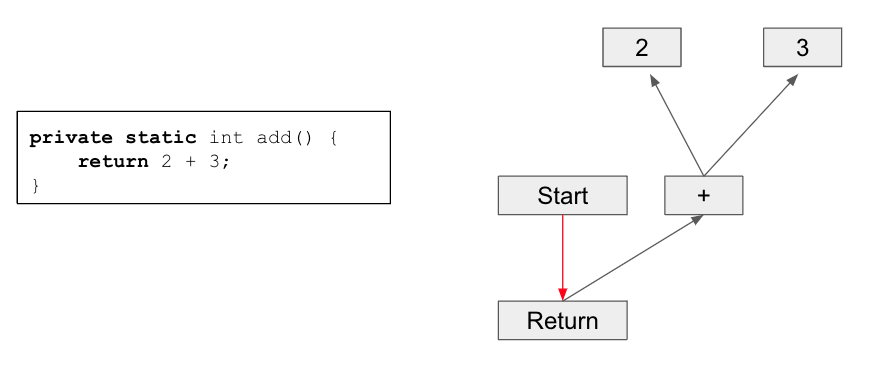
\includegraphics[width=1\textwidth]{Packages/graphir.png}
    \caption{Simple IR Graph}
    \label{figure:graphir}
\end{figure}

\autoref{figure:graphir} illustrates a simple IR graph, with control flow edges highlighted in red. The graph begins at the Start node, which connects to the Return node via a successor edge. Upon reaching the Return node, the graph traverses upward through data flow edges to compute the returned expression’s value. This traversal demonstrates how control and data flows interact to process and complete the function's execution.

\subsection{Prolog Programming Language}

In traditional imperative languages, a program consists of a sequence of instructions. This approach emphasizes a step-by-step procedure where each instruction modifies the state of the machine to solve a given problem. In contrast, logic programming languages, such as Prolog, operate on a fundamentally different paradigm. Instead of prescribing a sequence of operations, logic programming focuses on defining a knowledge base composed of facts and rules \cite{Bramer2013}. After that, users can query the knowledge base to search for objects and relations. 

In Prolog, facts represent objects and their relationships, while rules imply the relationship between objects given it satisfies all the conditions. Once the knowledge base is established, users can formulate queries to extract information or solve problems by leveraging the logical relationships defined in the base using the depth-first search algorithm \cite{Chowdhary2020}. There may be several ways to achieve a given goal. The system initially selects the first available option. If Prolog fails to resolve a specific subgoal, it will backtrack to explore these previously noted alternatives. This mechanism, referred to as backtracking \cite{Chowdhary2020}, enables Prolog to systematically search for different solutions by revisiting and trying alternative paths.

\begin{figure}[h]
    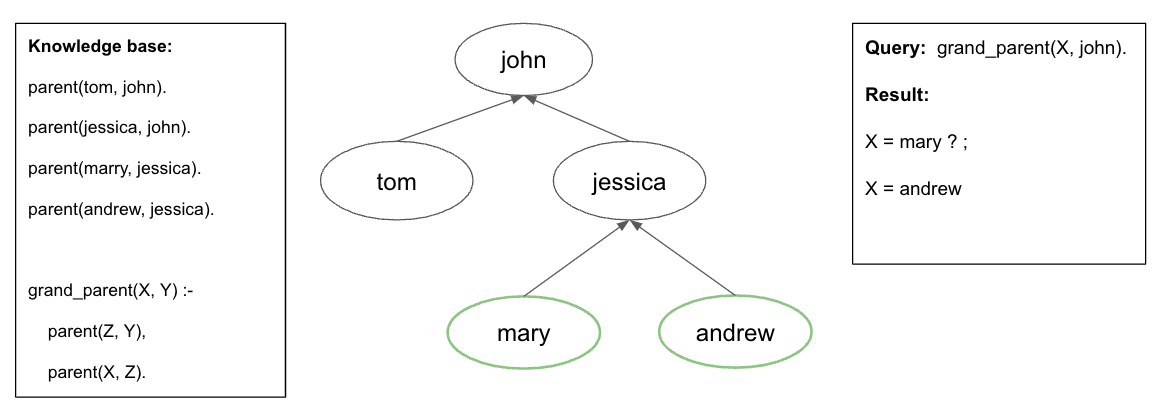
\includegraphics[width=0.95\textwidth]{Packages/Prolog.png}
    \caption{Example of Prolog specification}
    \label{figure:prolog}
\end{figure}

\autoref{figure:prolog}  illustrates a Prolog program. The first and final clauses are facts, specifying that nodeA is the parent of both nodeB and nodeC. In contrast, the intermediate clause represents a rule, which defines that nodeA is not the parent of nodeD. When a query is made to determine the nodes for which nodeA is a parent, Prolog executes a search from the first to the last clause, demonstrating its backtracking behavior.

\section{Literature Review}

\subsection{Advancements Through Domain-Specific Languages (DSLs)}
Declarative domain-specific languages (DSLs) have made a big impact on compiler optimization by offering targeted solutions for specific optimization tasks. For example, the Halide programming language improves image processing by separating the algorithm from its schedule, essentially the optimizations applied to the code \cite{Jonathan2018}. This separation allows for efficient and parallelized implementations with less manual effort. However, automating scheduling and keeping algorithms modular, especially as they grow in complexity, remains a challenge. Meanwhile, Spinellis created a peephole optimizer that uses a declarative DSL to specify optimizations \cite{Spinellis1999}. Spinellis transformed specifications into string regular expressions, which are then applied to the target code, allowing for adaptive and efficient refinements. Although this method has only been tested on smaller programs and specific types of optimizations so far, it shows great potential for quickly experimenting with new techniques and architectures. Elevate \cite{Hagedorn2020} is another functional language designed to let programmers define custom optimization strategies. It allows for creating composable optimizations rather than sticking to predefined APIs. Its success in case studies and practical applications highlights its ability to handle complex optimization tasks and deliver strong performance.

\subsection{Advancements Through Logic Programming Languages}
DataLog has established itself as a powerful tool in compiler implementation through its applications in complex program analysis and transformation. For instance, Lam et al. developed a framework using Datalog queries and a specialized language called PQL, which employs deductive databases and binary decision diagrams (BDDs) to tackle complex issues like pointer aliasing and heap object management in a context-sensitive manner \cite{Lam2005}. This approach has simplified the creation of sophisticated analyses and has been crucial in identifying security vulnerabilities in C and Java applications. Similarly, the Doop framework \cite{Bravenboer2009} utilizes Datalog to offer a declarative solution for points-to analysis in Java, providing impressive performance gains and scalability for precise context-sensitive analyses that were previously challenging to achieve. Furthermore, the Soufflé Datalog engine \cite{silverman2021wantanalyzeschemeprograms} introduces a new method for control-flow analysis in Scheme, making it possible to perform scalable and complex analyses of functional programming constructs, and extending the benefits of Datalog-based static analysis to Scheme-like languages. Finally, DIMPLE \cite{Benton2007}, a framework for Java bytecodes static analyses, is implemented in the Yap Prolog system. DIMPLE leverages logic programming capabilities to provide a declarative language for specifying analyses and representing Java bytecodes. The framework facilitates iterative experimentation and delivers efficient implementations that are on par with specialized tools.

\subsection{Transformation, Rewriting Techniques, and Verification}
Transformation and rewriting techniques are essential components of modern compiler optimization, enabling sophisticated processes like grammar specification, pattern matching, and program rewriting. Stratego \cite{Eelco2001} distinguishes between rewriting strategies and transformation rules, which allows for a highly flexible and controlled approach to applying optimization rules. The Stratego compiler translates these specifications into C code and leverages the ATerm library for effective term representation. It incorporates various optimizations, such as aggressive inlining and pattern merging, although it still encounters challenges related to compilation speed and support for separate compilation~\cite{Eelco2001}. On the other hand, Veriopt \cite{Webb2023} offers a comprehensive framework for formally verifying optimization rules used in the GraalVM compiler. This framework employs term rewriting rules on an abstract term representation and then maps these rules to term graph transformations. Veriopt has successfully validated 45 optimization rules for GraalVM’s intermediate representation, thus advancing the reliability and effectiveness of compiler optimizations.

\subsection{Identified Research Gaps}
Despite the established effectiveness of logic programming languages like Datalog in program analysis, there is limited research on integrating these techniques within modern compiler frameworks such as GraalVM. While significant advancements have been made in transformation and rewriting techniques using domain-specific languages (DSLs) and other paradigms, there is a notable absence of comparative studies on incorporating logic programming-based optimizations into GraalVM. This gap extends to a lack of empirical evidence assessing the impact of such techniques on optimization time and efficiency. Integrating Prolog-based rules with GraalVM’s graph-based IR is particularly challenging due to insufficient research on mapping Graal IR to Prolog and ensuring that Prolog-based optimizers work effectively within the Java environment. Addressing these challenges could enhance our understanding of how to apply logic programming in modern compilers and improve compiler optimization practices by providing valuable insights into the performance and effectiveness of these techniques.

\chapter[Literature Review]{Literature}

\section{Domain-Specific Languages (DSLs)}
Declarative domain-specific languages (DSLs) have made a big impact on compiler optimization by offering targeted solutions for specific optimization tasks. For example, Halide \cite{Jonathan2018} is a domain-specific language and compiler framework designed to optimize image processing and computational photography. Writing efficient code for image processing often requires complex optimizations to exploit parallelism and memory locality. In Halide, the algorithm specifies the computational logic for these tasks, detailing what needs to be done, such as resizing, sharpening, or blurring an image. The schedule defines the execution strategy, including how computations are ordered, parallelized, and managed in memory. This separation of concerns allows Halide to generate highly optimized code by focusing on both the functional description and the efficient execution of tasks. Elevate \cite{Hagedorn2020} is another functional language designed to let programmers define custom optimization strategies. It allows for creating composable optimizations rather than sticking to predefined APIs. Its success in case studies and practical applications highlights its ability to handle complex optimization tasks and deliver strong performance.

\begin{figure}[h]
    \centering
    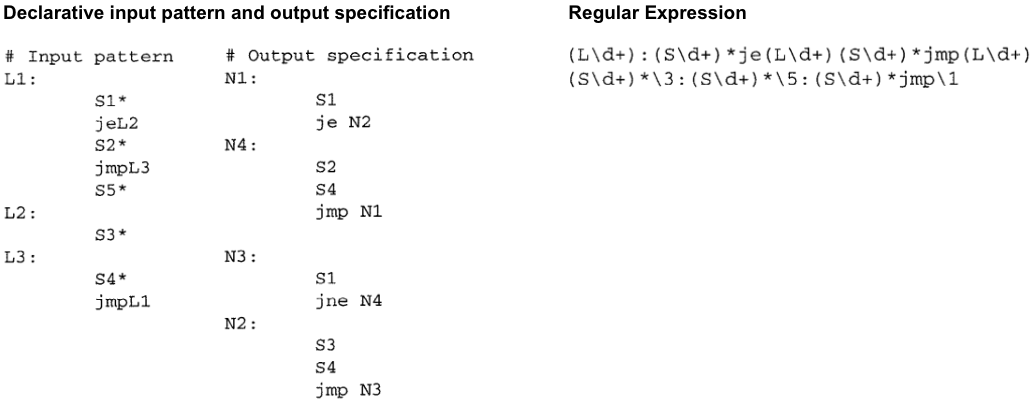
\includegraphics[width=1\textwidth]{Packages/regex.png}
    \caption{Example of Optimizer Patterns and Regular Expression \cite{Spinellis1999}}
    \label{figure:regex}
\end{figure}

Spinellis created a peephole optimizer that uses a declarative DSL to specify optimizations \cite{Spinellis1999}. Spinellis transformed specifications into string regular expressions, which are then applied to the target code, allowing for adaptive and efficient refinements. \autoref{figure:regex} illustrates an example of this framework. On the left of the figure is a declarative specification for the one-bit loop optimization \cite{Spinellis1999}. The input pattern is parsed and translated into the regular expression in the right part of the figure. The optimizer uses regular expressions to find matches in the program and transform and optimize the code iteratively.

\section{Logic Programming Languages}
DataLog has established itself as a powerful tool in compiler implementation through its applications in complex program analysis and transformation. For instance, the Soufflé Datalog engine \cite{silverman2021wantanalyzeschemeprograms} introduces a new method for control-flow analysis in Scheme, making it possible to perform scalable and complex analyses of functional programming constructs, and extending the benefits of Datalog-based static analysis to Scheme-like languages. Similarly, DIMPLE \cite{Benton2007}, a framework for Java bytecode static analyses, is implemented in the Yap Prolog system. DIMPLE leverages logic programming capabilities to provide a declarative language for specifying analyses and representing Java bytecodes. The framework facilitates iterative experimentation and delivers efficient implementations that are on par with specialized tools. 

Another example is the Doop framework \cite{Bravenboer2009} which utilizes Datalog to offer a declarative solution for points-to analysis in Java, providing impressive performance gains and scalability for precise context-sensitive analyses. \autoref{figure:doop} illustrates a Datadog rule that Doop uses to represent a call graph. The query finds and returns a call graph edge if all of the predicates inside \texttt{CallGraphEdge} are true. First, it queries the properties of the virtual method call \texttt{call} including its receive object \texttt{base}, \texttt{name}, and \texttt{descriptor}. After that, it queries the \texttt{heap} that this \texttt{base} object is pointing to and checks for the type of that \texttt{heap} object. Finally, it queries method lookups for the method that is being called from the \texttt{heaptype}.

\begin{figure}[h]
    \centering
    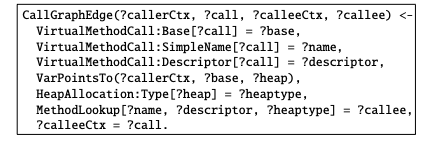
\includegraphics[width=0.6\textwidth]{Packages/Doop.png}
    \caption{DOOP's rule for virtual method invocations \cite{Bravenboer2009}}
    \label{figure:doop}
\end{figure}

Lam et al. developed a framework using Datalog queries and a specialized language called PQL, which employs deductive databases and binary decision diagrams (BDDs) to tackle complex issues like pointer aliasing and heap object management in a context-sensitive manner \cite{Lam2005}. PQL helps simplify the process by allowing programmers to write queries in a more intuitive way. Instead of needing to understand the underlying database details, programmers can write code patterns in Java that are automatically converted into Datalog. \autoref{figure:pql} provides an example of a query for simple SQL injection written in PQL and the equivalent Datadog rules. The SQL injection can be caught by checking if the parameter returned from calling \texttt{getParameter} on a \texttt{HttpServletRequest} is then passed directly as an argument to an \texttt{execution} call on the database \texttt{Connection}. Similarly, Datadog rules first check if there exists a method call to \texttt{getParameter} with a return value stored in a \texttt{v1} variable pointing to a heap object \texttt{h}. After that, it checks if there exists an invocation of \texttt{execute} with an argument \texttt{v2} also pointing to the object \texttt{h}.

\begin{figure}[h]
    \centering
    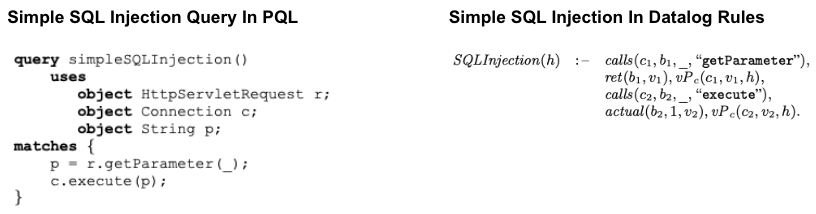
\includegraphics[width=1\textwidth]{Packages/PQL.png}
    \caption{Simple SQL Injection Example in PQL \cite{Lam2005}}
    \label{figure:pql}
\end{figure}

\newpage
\section{Transformation, Rewriting Techniques, and Verification}
Transformation and rewriting techniques are essential to modern compiler optimization, enabling sophisticated processes like grammar specification, pattern matching, and program rewriting. Stratego~\cite{Eelco2001} is a language designed for specifying program transformation systems using rewriting strategies, which allow for precise control over rule application. The compiler transforms these rules into C code and leverages the ATerm library for effective term representation. It has been used in several applications, including program transformation tools like XT, and domain-specific optimization frameworks like CodeBoost ~\cite{Eelco2001}. On the other hand, Veriopt \cite{Webb2023} offers a comprehensive framework for formal verification of Graal compiler optimizations. This framework employs  ``term rewriting rules on the abstract term representation" \cite{Webb2023} and then maps these rules to term graph transformations. In the Veriopt project, a term rewriting system, also known as an optimization phase, comprises a set of rules that can be applied repeatedly to optimize expressions. Each phase is associated with different types of root nodes in patterns, such as AddNode, AbsNode, and MulNode. 

\begin{figure}[h]
    \centering
    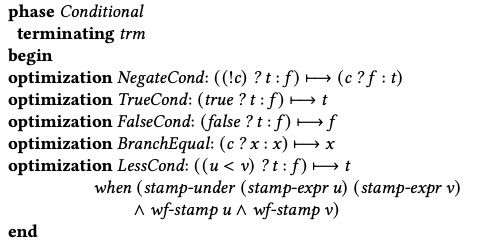
\includegraphics[width=0.6\textwidth]{Packages/veriopt.png}
    \caption{Conditional canonicalization rules \cite{Webb2023}}
    \label{figure:veriopt}
\end{figure}

\autoref{figure:veriopt} provides an example of such an optimization phase tailored for conditional expressions. NegateCond transforms negated conditions using logical equivalences, while TrueCond simplifies expressions where the condition is always true by directly applying the true outcome. Conversely, FalseCond addresses conditions that are always false by eliminating irrelevant branches. BranchEqual simplifies expressions with equality checks by optimizing or removing redundant comparisons.

\section{Identified Research Gaps}
Despite the established effectiveness of logic programming languages like Datalog in program analysis, there is limited research on integrating these techniques within modern compiler frameworks such as GraalVM. While significant advancements have been made in transformation and rewriting techniques using domain-specific languages (DSLs) and other paradigms, there is a notable absence of comparative studies on incorporating logic programming-based optimizations into GraalVM. This gap extends to a lack of empirical evidence assessing the impact of such techniques on optimization time and efficiency. Integrating Prolog-based rules with GraalVM’s graph-based IR is particularly challenging due to insufficient research on mapping Graal IR to Prolog and ensuring that Prolog-based optimizers work effectively within the Java environment. Addressing these challenges could enhance our understanding of how to apply logic programming in modern compilers and improve compiler optimization practices by providing valuable insights into the performance and effectiveness of these techniques.

\chapter[Implementation]{Implementation}
\section{IR to Prolog Translation}
To enable logic-based optimization in GraalVM, the intermediate representation (IR) must first be translated into a form that a Prolog engine can understand. This involves converting each IR node into a Prolog-compatible term that captures its structure and semantics. These terms can then be used as inputs to Prolog rules for reasoning and optimization, or asserted into the knowledge base when needed.
The representation is designed to be simple, uniform, and easy to parse. Each IR node is expressed as a term of the form \texttt{node(Id, Type, \ldots)}, where the first argument is a unique identifier for the node, and the second indicates its type (e.g., \texttt{add}, \texttt{if}, \texttt{constant}). The remaining arguments depend on the node type and encode operands, literal values, or successor relationships. This positional convention ensures that both data-flow and control-flow relationships are consistently represented and easily processed by Prolog.

\subsection*{Binay Arithmetic Nodes}
Binary arithmetic operations such as addition, subtraction, and similar computations are represented using the following structure:

\begin{lstlisting}[language=Prolog]
node(Id, Type, FirstOperandId, SecondOperandId)
\end{lstlisting}

Where:
\begin{itemize}
\item \texttt{Id}: Unique identifier for this node.
\item \texttt{Type}:  Specifies the arithmetic operation being performed (e.g., \texttt{add}, \texttt{sub}).
\item \texttt{FirstOperandId} and \texttt{SecondOperandId}: Identifiers of the nodes providing the operands.
\end{itemize}

\textbf{Example:}
\begin{lstlisting}[language=Prolog]
node(1, add, 2, 3)
\end{lstlisting}
This defines an \texttt{AddNode} with ID \texttt{1}, which computes the sum of the results from nodes \texttt{2} and \texttt{3}.


\subsection*{Control Flow Nodes}

Control flow constructs, such as conditional branches, are represented as follows:

\begin{lstlisting}[language=Prolog]
node(Id, Type, ConditionId, TrueSuccessorId, FalseSuccessorId)
\end{lstlisting}

Where:
\begin{itemize}
  \item \texttt{Id}: Unique identifier for this control node.
  \item \texttt{Type}: Specifies the control type (e.g., \texttt{if}, \texttt{while}).
  \item \texttt{ConditionId}: Identifier of the node that evaluates the condition.
  \item \texttt{TrueSuccessorId}: Node to proceed to if the condition is true.
  \item \texttt{FalseSuccessorId}: Node to proceed to if the condition is false.
\end{itemize}

\textbf{Example:}
\begin{lstlisting}[language=Prolog]
node(1, if, 2, 3, 4)
\end{lstlisting}
This defines an \texttt{IfNode} with ID \texttt{1}, which evaluates the condition from node \texttt{2}. If the condition is true, control flows to node \texttt{3}; otherwise, it flows to node \texttt{4}.

\bigskip

The translation process is implemented by extending the \texttt{toString} method of each IR node class to support a new verbosity level: \texttt{Verbosity.Prolog}. When this verbosity level is selected, each node formats itself as a Prolog-compatible term that reflects its internal structure and relationships. This approach leverages GraalVM's existing verbosity mechanism, which allows nodes to produce different string representations depending on the context.
By introducing the \texttt{Prolog} verbosity level, IR nodes can emit a consistent, structured representation that is suitable for use as input to Prolog rules or for assertion into the logic engine. The following code snippet illustrates how the \texttt{toString} method of the \texttt{IfNode} class was extended to support this additional verbosity level:

\begin{lstlisting}[language=Java]
@Override
public String toString(Verbosity verbosity) {
    if (verbosity == Verbosity.Prolog) {
        return "node(" + String.join(
                ",",
                toString(Verbosity.Id),
                toString(Verbosity.Name).toLowerCase(),
                condition.toString(Verbosity.Id),
                trueSuccessor.toString(Verbosity.Id),
                falseSuccessor.toString(Verbosity.Id)
        ) + ")";
    } else {
        return super.toString(verbosity);
    }
}
\end{lstlisting}

\section{Prolog Optimization Rules}
\label{sec:rules}
Each optimization in this framework is defined in a Prolog file named after the transformation it performs, such as \texttt{addNode.pl}.
These files contain the logic rules that describe how specific intermediate representation (IR) patterns should be recognized and transformed during compilation.
Stateless optimizations such as canonicalization and loop invariant reassociation are purely pattern based.
They operate by matching structural patterns in the IR and returning transformed results without modifying the knowledge base.
In contrast, stateful optimizations such as conditional elimination require tracking intermediate state during query execution.
These optimizations use Prolog’s dynamic capabilities, including fact assertion and retraction, to simulate data flow and propagate information such as possible kwown variable values for conditional elimination optimization.

\lstset{
    aboveskip=5pt,
    belowskip=5pt
}
\subsection{Add Node Canonicalization}
\subsection*{Use cases}
This project has implemented eight exploratory canonicalization rules for the \texttt{AddNode} as shown below.
\begin{align*}
    x + (-y)          &\rightarrow x - y        &\qquad -x + y           &\rightarrow y - x \\
    \sim x + x        &\rightarrow -1           &\qquad x + \sim x       &\rightarrow -1     \\
    x + 0             &\rightarrow x            &\qquad 0 + x            &\rightarrow x      \\
    (x - y) + y       &\rightarrow x            &\qquad x + (y - x)      &\rightarrow y      \\
\end{align*}
These rules target common arithmetic simplifications that occur in real-world programs and can lead to more efficient generated code by eliminating unnecessary operations.
Canonicalization is particularly valuable because it tends to expose further optimization opportunities and simplify control or data flow in the IR.
The Prolog rules for these transformations are simple and stateless, making them well-suited for logic-based, declarative expressions.
This declarative form makes the rules easy to read and reason about.

\subsection*{Prolog Implementation}
\begin{lstlisting}[language=Prolog]
% (x - y) + y -> x
canonical(node(add, node(Id, sub, IdX, IdY), IdY), Result) :-
   Result = lookup(IdX).
\end{lstlisting}
    
This rule matches an \texttt{addnode} where the first operand is a \texttt{subnode} identified by \texttt{Id}, and the second operand is identical to the right operand of that subtraction. The transformation relies solely on node identifiers rather than the internal structure of the nodes. When the same node ID \texttt{IdY} appears both as the right operand of the subtraction and as the second operand of the addition, the rule simplifies the expression \texttt{(x - y) + y} to just \texttt{x} by returning a lookup of \texttt{IdX}. Using node identifiers works correctly because the intermediate representation employs common subexpression sharing and global value numbering, ensuring that identical subexpressions share the same node ID. The resulting structure is returned as a new term in the variable \texttt{Result}, which is later parsed and reconstructed back into a GraalVM IR node by the result parser.

\subsection*{Java Implementation Comparision}
\begin{lstlisting}[language=Java]
if (forX instanceof NegateNode) {
    // -x + y => y - x
    return BinaryArithmeticNode.sub(forY, ((NegateNode) forX).getValue(), view);
} else if (forY instanceof NegateNode) {
    // x + -y => x - y
    return BinaryArithmeticNode.sub(forX, ((NegateNode) forY).getValue(), view);
} ...
\end{lstlisting}

The code snippet above provides example of the Java implementation for canonicalization rules.
Both the Java and Prolog versions aim to perform arithmetic simplification, and in this case, both are relatively simple because the underlying transformation rule itself is straightforward. 
However, the Prolog version stands out in terms of expressiveness and clarity. The Java code, while easy to follow, relies on verbose type checking and manual unwrapping of nodes, using imperative control flow and explicit casting to express the rule. In contrast, the Prolog version concisely encodes the same transformation using a single declarative clause that mirrors the algebraic identity directly. This leads to greater readability and a closer correspondence between the code and the mathematical reasoning behind the optimization, making the intent of the transformation immediately apparent.
\lstset{
    aboveskip=0pt,
    belowskip=0pt
}
\subsection{And Node Canonicalization}
\subsection*{Use cases}
This project has implemented two canonicalization rules for the \texttt{AndNode} as shown below.
\begin{align*}
    x \,\&\, y &\rightarrow y \quad \text{if } \sim \texttt{mustSetX} \,\&\, \texttt{maySetY} = 0 \\
    x \,\&\, y &\rightarrow x \quad \text{if } \sim \texttt{mustSetY} \,\&\, \texttt{maySetX} = 0
\end{align*}

These rules, while still stateless and pattern-based, are slightly more involved than typical structural rules because they depend on semantic properties of the operands. Specifically, they require inspecting the \texttt{mustSet} and \texttt{maySet} bitmasks associated with the operands. In the context of compiler optimizations, \texttt{mustSet} and \texttt{maySet} are abstract representations of known and possible values at the bit level. The \texttt{mustSet} bitmask identifies bits that are guaranteed to be 1 in the operand, while the \texttt{maySet} bitmask identifies bits that could potentially be 1. These bitmasks enable reasoning about the outcome of bitwise operations without knowing exact operand values at compile time.
These rules help reduce redundant operations and enable further simplifications by eliminating unnecessary bitwise computations when the operand properties make them semantically redundant.

\subsection*{Prolog Implementation}
\begin{lstlisting}[language=Prolog]
% Complement of a bitmask
bitwise_not(X, Result) :-
    Mask is (1 << 32) - 1,
    Result is X xor Mask.

% x & y -> y if ~mustBeSetX & mayBeSetY == 0
canonical(node(andnode, X, Y, StampX, StampY), Result) :-
    StampX = stamp(_, _, MustBeSetX, _,),
    StampY = stamp(_, _, _, MayBeSetY),
    bitwise_not(MustBeSetX, ComplementMustBeSetX),
    (ComplementMustBeSetX /\ MayBeSetY) = 0,
    find_id(Y, IdY),
    Result = lookup(IdY).
\end{lstlisting}
This rule matches an \texttt{andnode} where the bitwise AND operation can potentially be simplified based on the bitmask metadata of its operands. 
It takes as input an \texttt{andnode} term consisting of two operand nodes along with their associated \texttt{stamp} information. 
Each \texttt{stamp} contains four pieces of data: minimum value that the node could have, maximum value that the node could have, \texttt{mustBeSet} bits, and \texttt{mayBeSet} bits. 
For this rule, only the \texttt{mustBeSet} and \texttt{mayBeSet} fields are relevant. 
The rule computes the bitwise complement of the first operand’s \texttt{mustBeSet} bits and then performs a bitwise AND with the second operand’s \texttt{mayBeSet} bits. 
If this result is zero, it indicates that the original AND operation can be simplified to just the second operand. 
The rule then extracts the unique identifier of this operand and returns it as the simplified result. 
The bitwise complement operation is implemented using a helper predicate \texttt{bitwise\_not} because the Projog engine does not provide a built-in predicate for this operation. 
This method leverages precise bit-level information to safely optimize the code.
A similar predicate is used to handle the complementary case where x is returned instead of y.
\subsection*{Java Implementation Comparision}
\begin{lstlisting}[language=Java]
IntegerStamp xStamp = (IntegerStamp) rawXStamp;
IntegerStamp yStamp = (IntegerStamp) rawYStamp;
if (((~xStamp.mustBeSet()) & yStamp.mayBeSet()) == 0) {
    return forY;
} else if (((~yStamp.mustBeSet()) & xStamp.mayBeSet()) == 0) {
    return forX;
}
\end{lstlisting}
The code snippet above provides the Java implementation for canonicalization rules.
Both the Java and Prolog versions implement the same underlying logic for the canonicalization of the bitwise AND operation, but they reflect their respective language paradigms in different ways. The Java code uses a single if-else statement to handle complementary cases within one procedural block, making the control flow explicit and linear. Meanwhile, the Prolog version expresses these cases as separate predicates, each capturing a specific rule declaratively. This separation aligns with Prolog’s logical programming style, allowing each case to be reasoned about independently. While the Prolog code is somewhat longer, it offers clarity through modular rules. Both approaches have similar control flow, but the expression differs to suit the strengths of each language.

\subsection{Loop Invariant Reassociation}
\subsection*{Use cases}
This project has implemented rules to match a variety of loop invariant reassociation patterns, as shown below.
\begin{align*}
    inv1 - (i + inv2)          &\rightarrow (inv1 - inv2) - i        &\qquad (i + inv2) - inv1           &\rightarrow i + (inv2 - inv1) \\
    (inv2 - i) + inv1          &\rightarrow (inv1 + inv2) - i        &\qquad (i - inv2) + inv1           &\rightarrow i + (inv1 - inv2) \\
    inv1 - (inv2 - i)          &\rightarrow i + (inv1 - inv2)        &\qquad inv1 - (i - inv2)           &\rightarrow (inv1 + inv2) - i \\
    (inv2 - i) - inv1          &\rightarrow (inv2 - inv1) - i        &\qquad (i - inv2) - inv1           &\rightarrow i - (inv1 + inv2) \\
    &\qquad  (i  \texttt{{\ }Op{\ }} inv2) \texttt{{\ }Op{\ }} inv1         &\rightarrow i \texttt{{\ }Op{\ }} (inv1 \texttt{{\ }Op{\ }} inv2) \\
\end{align*}
In these patterns, \texttt{inv1} and \texttt{inv2} represent invariant expressions that do not change within the loop, while \texttt{i} denotes a loop-variant variable. The goal of these rules is to isolate the loop-variant component in order to enable hoisting of loop-invariant computations outside the loop.
The last rule in the table represents a generalized reassociation pattern where both occurrences of the operator \texttt{Op} must be the same and drawn from a specific set of associative operations: addition, multiplication, bitwise AND, OR, XOR, and arithmetic max or min. 
These operations are associative and commutative, meaning the order of operands does not affect the result.

\subsection*{Prolog Implementation}
\begin{lstlisting}[language=Prolog]
% Entry point for invariant reassociation   
find_reassociate_inv(Node, LoopNodes, R) :-
    node_type(Node, NodeType, X, Y, IdX, IdY),
    find_reassociate(
        X, Y, IdX, IdY, 
        LoopNodes, Match1Id, Other1, MatchSide1
    ),
    node_type(
        Other1, Other1Type, Other1X, Other1Y, 
        Other1XId, Other1YId
    ),
    find_reassociate(
        Other1X, Other1Y, Other1XId, Other1YId, 
        LoopNodes, Match2Id, Other2, MatchSide2
    ),
    find_id(Other1, Other1Id),
    find_id(Other2, Other2Id),
    reassociate_rule(
        NodeType, Other1Type, Match1Id, Match2Id, 
        MatchSide1, MatchSide2, Other2Id, R
    ).
\end{lstlisting}

The predicate \texttt{find\_reassociate\_inv/3} serves as the entry point for identifying potential opportunities to reassociate invariant computations. The predicate takes a node (\texttt{Node}), a list of loop-related nodes (\texttt{LoopNodes}), and returns a reassociation result (\texttt{R}). It begins by extracting the type and subcomponents of the input node via \texttt{node\_type/6}. It then attempts to find a matching reassociation pattern for the first level of operands using \texttt{find\_reassociate/7}, which yields a matched node identifier (\texttt{Match1Id}), the non-matching "other" node (\texttt{Other1}), and which side the match occurred on (\texttt{MatchSide1}). The process is repeated for \texttt{Other1}, attempting to trace a second level of potential reassociation. The identifiers for these "other" nodes are resolved using \texttt{find\_id/2}, and finally, all gathered information is passed into \texttt{reassociate\_rule/8}, which checks whether a valid transformation rule applies and produces the reassociation result (\texttt{R}). Unlike the canonicalization rule, which typically operates on a single node in isolation, this rule explores a chain of connected nodes.
\smallbreak
\begin{lstlisting}[language=Prolog]
% Base case: NodeId should not be in LoopNodes.
is_invariant(Node, NodeId, LoopNodes) :-
    \+ member(NodeId, LoopNodes).

% Recursive case: Check invariants for the children nodes X and Y.
is_invariant(Node, NodeId, LoopNodes) :-
    node_type(Node, NodeType, X, Y, IdX, IdY),
    is_invariant(X, IdX, LoopNodes),
    is_invariant(Y, IdY, LoopNodes).

% Case: Left is invariant, Right is variant
find_reassociate(X, Y, IdX, IdY, LoopNodes, IdX, Y, left) :-
    is_invariant(X, IdX, LoopNodes),
    \+ is_invariant(Y, IdY, LoopNodes).

% Case: Right is invariant, Left is variant
find_reassociate(X, Y, IdX, IdY, LoopNodes, IdY, X, right) :-
    \+ is_invariant(X, IdX, LoopNodes),
    is_invariant(Y, IdY, LoopNodes).
\end{lstlisting}

\smallbreak
The above Prolog code defines logic for identifying loop-invariant computations and potential reassociation opportunities. The predicate \texttt{is\_invariant/3} determines whether a node is invariant with respect to a list of loop-related node identifiers given by \texttt{LoopNodes}. In the base case, a node is considered invariant if its identifier, \texttt{NodeId}, is not a member of \texttt{LoopNodes}. In the recursive case, the predicate assumes the node has two child nodes, \texttt{X} and \texttt{Y}, with corresponding identifiers \texttt{IdX} and \texttt{IdY}. It recursively checks that both children are invariant. The predicate \texttt{find\_reassociate/7} defines cases for recognizing expressions where one side is invariant and the other is not. In the first case, if the left child \texttt{X} is invariant and the right child \texttt{Y} is not, then it identifies \texttt{X} as the match and sets the side to \texttt{left}. In the second case, if the right child \texttt{Y} is invariant and the left child \texttt{X} is not, then it identifies \texttt{Y} as the match and sets the side to \texttt{right}. 
This logic enables detection of partial invariant expressions that could be reassociated to improve performance.

\smallbreak
\begin{lstlisting}[language=Prolog]
% Rule for addnode with subnode
reassociate_rule(
    addnode, subnode, Match1Id, Match2Id, 
    MatchSide1, MatchSide2, Other2Id, R
) :-
    reassociate_add_sub(Match1Id, Match2Id, Other2Id, MatchSide2, R).
\end{lstlisting}
\smallbreak
The above Prolog code defines a specific pattern-matching rule for reassociating arithmetic expressions in the case where the first operation is addition and the second operation is subtraction. The predicate \texttt{reassociate\_rule/8} captures this transformation by invoking \texttt{reassociate\_add\_sub/5}, which encodes two concrete transformation patterns.
The \texttt{reassociate\_rule/8} predicate takes as input the types of the first and second operations (e.g., \texttt{addnode} and \texttt{subnode}), the identifiers of two matched subexpressions (\texttt{Match1Id} and \texttt{Match2Id}), information about which sides of the expressions matched (\texttt{MatchSide1} and \texttt{MatchSide2}), the identifier of the other node involved in the reassociation (\texttt{Other2Id}), and finally returns the reassociated expression \texttt{R}. This input allows \texttt{reassociate\_rule/8} to select and apply the appropriate transformation pattern based on the structure and position of the invariant subexpressions.

\smallbreak
\begin{lstlisting}[language=Prolog]
% (inv2 - i) + inv1 -> (inv1 + inv2) - i
reassociate_add_sub(
    Match1Id, Match2Id, Other2Id, left,
    node(
        subnode, 
        node(addnode, lookup(Match1Id), lookup(Match2Id)), 
        lookup(Other2Id))
    ).

% (i - inv2) + inv1 -> i + (inv1 - inv2)
reassociate_add_sub(
    Match1Id, Match2Id, Other2Id, right,
    node(
        addnode, 
        node(subnode, lookup(Match1Id), lookup(Match2Id)), 
        lookup(Other2Id))
    ).
\end{lstlisting}

\smallbreak
The two clauses of \texttt{reassociate\_add\_sub/5} define transformation rules that restructure arithmetic expressions to group loop-invariant computations. The first clause handles the case where the second invariant appears on the left side of a subtraction, while the second clause deals with the scenario where the invariant is on the right. In both cases, the transformation rearranges the expression so that the invariant parts are grouped together. 
This is just one example of a family of rules used to optimize expressions through reassociation. Similar predicates exist for other operator combinations such as \texttt{reassociate\_sub\_sub}, \texttt{reassociate\_sub\_add}, and so on, each encoding the specific transformation rules for their respective operator pairings.

\subsection*{Java Implementation Comparision}

\begin{lstlisting}[language=Java]
ValueNode m1 = match1.getValue(node);
ValueNode m2 = match2.getValue(other);
ValueNode a = match2.getOtherValue(other);
if (isNonExactAddOrSub(node)) {
    ValueNode associated;
    if (invertM1) {
        associated = BinaryArithmeticNode.sub(m2, m1, view);
    } else if (invertM2) {
        associated = BinaryArithmeticNode.sub(m1, m2, view);
    } else {
        associated = BinaryArithmeticNode.add(m1, m2, view);
    }
    if (invertA) {
        return BinaryArithmeticNode.sub(associated, a, view);
    }
    if (aSub) {
        return BinaryArithmeticNode.sub(a, associated, view);
    }
    return BinaryArithmeticNode.add(a, associated, view);
}
...
\end{lstlisting}

The code snippet above provides the Java implementation for reassociating invariant in loop.
Both the Java and Prolog implementations perform loop invariant reassociation but differ significantly in style and clarity. The Java version uses several intermediary boolean variables like \texttt{invertM1}, \texttt{invertM2}, and \texttt{aSub} to control the flow and decide which arithmetic operation to apply. This approach, while compact, can be harder to follow because the logic is spread across multiple conditions and temporary variables, making the reasoning less direct. In contrast, the Prolog version is generally longer since it encodes each specific reassociation case as a separate predicate clause. This explicit case-by-case structure makes the Prolog code easier to understand and reason about, as each rule clearly corresponds to a particular algebraic transformation without relying on mutable state or complex branching.
\subsection{Conditional Eliminationtion}
\subsection*{Use cases}
This project has implemented rules to match a variety of condtional elimination cases, examples of which are shown below.
\smallbreak

\begin{lstlisting}
// Case 1: X equals a constant
if (x == 1) {
    // this block is simplified to false
    if (x == 2) {}
}
// Case: 2: X is larger than a constant
if (x > 1) {
    // this block is simplified to false
    if (x == 0) {}
}
\end{lstlisting}

The Prolog rules for conditional elimination represent the most stateful and structurally complex analysis in this project. Unlike previous optimizations, which are generally stateless and operate locally on individual nodes, conditional elimination must track and manage global control flow context throughout the analysis. The underlying intermediate representation graph is structured according to a dominator tree, which describes which nodes dominate others in the control flow. However, this tree does not provide a direct parent and child relationship that is easily accessible. Therefore, the analysis cannot rely solely on static relationships; it must dynamically assert and retract facts that describe current conditions and known variable states as it traverses the dominator tree.

A central concept in this analysis is the stamp. A stamp represents the known value range of a variable at a certain point in the control flow, typically recorded as a lower and upper bound. In addition to the bounds, each stamp also records the identifier of the node where the value range was derived. This allows the analysis to later determine the scope of that information and retract it when it becomes invalid. Stamps are inferred from control flow conditions. For example, if the analysis encounters a branch that only executes when the variable x is less than five, it can assert a stamp recording that the value of x must be less than five on that path, and that this constraint originates from the current conditional node. These known ranges are later used to simplify or eliminate subsequent conditional expressions, allowing the system to reason more effectively about the program’s behavior.

Because the analysis moves down through the dominator tree and later back up, the state must be carefully managed. When descending into a node, new stamps may be asserted to reflect updated knowledge about variable values. However, when the traversal moves upward again, those stamps must be retracted to avoid applying invalid assumptions to unrelated parts of the graph. This stateful approach ensures that the analysis remains sound and accurate, while still enabling powerful optimizations such as the elimination of unreachable branches and the simplification of guarded conditions.

\subsection*{Prolog Implementation}
\begin{lstlisting}[language=Prolog]
// Entry predicate for processing if nodes
process_if_nodes(Node, Result) :-
    node(NodeId, if, _, _, _),
    update_state(NodeId, DominatorId),
    check_successor_type(NodeId, DominatorId, SuccType),
    check_guard(NodeId, DominatorId, SuccType),
    try_fold(NodeId, DominatorId, SuccType, Result),
    Node = lookup(NodeId).
\end{lstlisting}

The predicate \texttt{process\_if\_nodes/2} identifies and processes all nodes in the knowledge base that represent conditional branches, i.e., nodes of type \texttt{if}. It does not take a specific input node but instead searches through the facts to find nodes matching the pattern \texttt{node(NodeId, if, \_, \_, \_)}.
For each such node, it updates the analysis state by determining the dominator node via \texttt{update\_state/2}, which finds the controlling predecessor in the control flow graph. It then examines the type of successor nodes related to this dominator using \texttt{check\_successor\_type/3}, and inspects the guarding conditions with \texttt{check\_guard/3}. Based on these checks, \texttt{try\_fold/4} attempts to simplify or fold the conditional node.  When \texttt{process\_if\_nodes/2} is queried, it systematically returns pairs of \texttt{NodeId} and \texttt{Result}, such as \texttt{(NodeId = 1, Result=node(boolean, false))}, reflecting the outcome of attempting to optimize each conditional branch.

\smallbreak
\begin{lstlisting}[language=Prolog]
% Predicate to find dominator of a block
find_dominator(NodeId, DominatorId) :-
    block(_, _, NodeId, DominatorBlockId),
    block(DominatorBlockId, _, DominatorId, _).

% Update child node level
update_child_level(ParentNodeId, ChildNodeId) :-
    level(ParentNodeId, Level),
    NewLevel is Level + 1,
    asserta_unique(level(ChildNodeId, NewLevel)).

% Update global state
update_state(NodeId, DominatorId) :-
    find_dominator(NodeId, DominatorId) ->
    (
        % Update node level and retract stale stamp
        update_child_level(DominatorId, NodeId),
        retract_stale_stamps(NodeId)
    );
    % First if node doesn't have a dominator
    asserta_unique(level(NodeId, 0)),
    fail.
\end{lstlisting}
\smallbreak
When visiting a new node, the \texttt{update\_state/2} coordinates process to find the node dominator, its level in the tree and retract stale stamps. First, it attempts to find its dominator. 
The predicate \texttt{find\_dominator/2} finds the immediate dominator of a node by looking up the block information: it first finds the block containing the \texttt{NodeId} and retrieves its dominator block, then finds the node corresponding to that dominator block, returning its identifier as \texttt{DominatorId}. 
Once the dominator is found, \texttt{update\_child\_level/2} updates the child node’s level relative to its parent by fetching the parent’s current level, incrementing it by one, and recording this new level for the child node using \texttt{asserta\_unique/1}. 
If no dominator is found (such as for the root or first \texttt{if} node), it assigns level zero to the node and returns failure. 
This mechanism tracks the depth of nodes in the dominator tree or control flow hierarchy, which is critical for later analysis or optimizations.
\smallbreak
\begin{lstlisting}[language=Prolog]
% Predicate to find the maximum value of levels
find_max_level(MaxLevel) :-
    findall(Level, level(_, Level), Levels),
    max_list(Levels, MaxLevel).

% Retract all stamps that are guarded by the lower node level
retract_stale_stamps(NodeId) :-
    level(NodeId, MinLevel),
    find_max_level(MaxLevel),
    findall(Num, between(MinLevel, MaxLevel, Num), StaleLevels),
    retract_stamps(StaleLevels).
retract_stamps([]).
retract_stamps([Level|Rest]) :-
    retractall(stamp(_, _, _, Level)),
    retract_stamps(Rest).
\end{lstlisting}

\smallbreak
To ensure consistency in the analysis, stale or outdated information about nodes lower in the dominator tree must be removed when visiting a new node. The predicate \texttt{retract\_stale\_stamps/1} achieves this by first determining the level of the current node, then finding the maximum node level recorded so far. It collects all levels between the current node’s level and the maximum and retracts all corresponding \texttt{stamp/4} facts for those levels, effectively clearing cached data that may no longer be valid due to new information higher in the tree.

\smallbreak

\begin{lstlisting}[language=Prolog]
% Predicate to check if a node is a true successor or a false successor of a given node
check_successor_type(NodeId, DominatorId, Result) :-
    node(DominatorId, if, TrueSucc, FalseSucc, _),
    node(TrueSucc, begin, NodeId) -> Result = true;
    node(FalseSucc, begin, NodeId) -> Result = false;
    Result = unknown.
\end{lstlisting}

\newpage
The above Prolog predicate \texttt{check\_successor\_type/3} determines whether a given \texttt{NodeId} is a true successor, a false successor, or neither (unknown) with respect to an \texttt{if} node identified by \texttt{DominatorId}. It starts by retrieving the \texttt{if} node corresponding to \texttt{DominatorId}, which has two successor nodes: \texttt{TrueSucc} and \texttt{FalseSucc}. Then it checks if the given \texttt{NodeId} matches the beginning node of the true branch (\texttt{TrueSucc}); if so, it binds \texttt{Result} to \texttt{true}. Otherwise, it checks if \texttt{NodeId} matches the beginning node of the false branch (\texttt{FalseSucc}); if so, it binds \texttt{Result} to \texttt{false}. If neither condition holds, it assigns \texttt{Result} to \texttt{unknown}.

\smallbreak
\begin{lstlisting}[language=Prolog]
check_guard(DomOp, IdX, DomValueY, SuccType, NodeId) :-
    % Do nothing if dominator value is null
    DomValueY == null -> true;
    (
        level(NodeId, GuardId),
        member(DomOp,['==']), SuccType == true
            -> asserta_unique(stamp(IdX, DomValueY, DomValueY, GuardId));
        member(DomOp,['<']), SuccType == false
            -> asserta_unique(stamp(IdX, DomValueY, max_int, GuardId));
        true
    ).

% check case both conditions are binary conditions,
% have the same node x, and y of the dominator condition is a constant
check_guard(NodeId, DominatorId, SuccType) :-
    node(NodeId, if, _, _, ConditionId),
    node(ConditionId, _, IdX, _),
    node(IdX, parameter(_)),
    node(DominatorId, if, _, _, DominatorConditionId),
    node(DominatorConditionId, DominatorOp, IdX, DominatorY),
    node(DominatorY, constant(DominatorYValue, _)),
    check_guard(DominatorOp, IdX, DominatorYValue, SuccType, NodeId).
\end{lstlisting}
\smallbreak
The above Prolog code is designed to recognize and remember useful information from conditional checks in earlier parts of a program’s control flow, which can later help optimize the program. The first predicate, \texttt{check\_guard/3}, operates at a higher level by examining the current node’s condition and its dominator’s condition. It ensures both conditions relate to the same variable with identifier \texttt{IdX} and that the dominator’s condition compares that variable to a constant. If these checks pass, it calls \texttt{check\_guard/5} to attempt recording a \texttt{stamp} representing the possible known variable values.
The second predicate, \texttt{check\_guard/5}, takes the comparison operator from the dominator node, the variable’s identifier \texttt{IdX}, the constant value \texttt{DomValueY} from the dominator node, the type of successor branch (true or false), and the current node \texttt{NodeId}. It first skips processing if the dominator value is missing. Otherwise, it retrieves the node’s level in the control flow and, based on the operator and successor type, records a \texttt{stamp} fact. For example, if the operator is equality and the branch is true, it records that the variable equals the constant. If the operator is less-than and the branch is false, it records that the variable is at least the constant value. This \texttt{stamp} acts as a fact that the system can later use to simplify expressions or optimize code.

\smallbreak
\begin{lstlisting}[language=Prolog]
% Constant condition: value stamp available and deterministic
try_fold('>=', ValueY, MinX, MaxX, true) :- 
    ValueY \= null, MinX == MaxX, MinX >= ValueY.
try_fold('>=', ValueY, MinX, MaxX, false) :- 
    ValueY \= null, MinX == MaxX, MinX < ValueY.
...
try_fold(_, ValueY, _, _, unknown) :- ValueY \= null.
try_fold(_, ValueY, _, _, unknown) :- ValueY == null.
try_fold(_, _, _, _, unknown).  % General fallback

% try fold the condition
try_fold(NodeId, DominatorId, SuccType, Result) :-
    node(NodeId, if, _, _, ConditionId),
    node(DominatorId, if, _, _, DominatorConditionId),
    node(ConditionId, Op, IdX, IdY),
    node(DominatorConditionId, DominatorOp, IdX, DominatorY),
    node(IdX, parameter(_)),
    node(IdY, constant(ValueY, _)),
    node(DominatorY, constant(DominatorYValue, _)),
    (
        stamp(IdX, MinX, MaxX, _) ->
            try_fold(Op, ValueY, MinX, MaxX, Result);
    ).
\end{lstlisting}
\smallbreak
The above Prolog code attempts to simplify or “fold” conditional expressions by using known constant value ranges to decide the truth of conditions. The predicate \texttt{try\_fold/4} serves as the entry point: it extracts the operator and operands from the current conditional node and its dominator node, ensuring both involve the same variable \texttt{IdX} and that the compared values are constants. It then looks up any known value range for \texttt{IdX} stored as a \texttt{stamp}. If such a range exists, \texttt{try\_fold/4} calls the more specific \texttt{try\_fold/5} predicate to attempt to evaluate the condition conclusively as \texttt{true}, \texttt{false}, or \texttt{unknown}. \texttt{try\_fold/5}, defines specific cases for different operators such as \texttt{'>='}. For example, if the operator is \texttt{'>='}, the constant \texttt{ValueY} is not null, and the known value range for the variable is a single value (\texttt{MinX} equals \texttt{MaxX}), then it returns \texttt{true} if that value satisfies the condition or \texttt{false} otherwise. Other operators have similar specialized rules. If none of these match, the predicate defaults to \texttt{unknown}, indicating the condition cannot be conclusively evaluated.

\subsection*{Java Implementation Comparision}
Both the Prolog and Java implementations of conditional elimination are inherently complex due to the nature of the analysis, involving intricate state tracking and control flow reasoning. The Java version typically spans multiple classes and methods, spreading the logic across different parts of the codebase, which can make following the overall flow challenging without jumping between files. In contrast, the Prolog implementation, while lengthy, expresses the logic declaratively within a set of predicates, making the reasoning about pattern matching and rule application more direct. However, Prolog’s declarative style may require understanding predicate dependencies and backtracking, which can be less intuitive for those unfamiliar with logic programming. Overall, both versions balance complexity differently: Java through imperative, object-oriented constructs with explicit state management, and Prolog through concise logical rules with implicit control flow.
\section{Query Result Parser}
A critical part of integrating Prolog-based optimization into the GraalVM compilation pipeline is interpreting the results of Prolog queries in a way that can be applied back to the compiler’s intermediate representation (IR). This task is handled by a custom Prolog result parser, which translates the Prolog engine’s output terms into corresponding GraalVM IR node constructions. The parser is implemented using a recursive descent approach and is designed to be modular, extensible, and robust to varying term structures. After optimization opportunities are identified through Prolog queries, the results returned by the logic engine must be interpreted as transformations to be applied to the IR graph. These transformations can include the reuse of existing nodes or the creation of new computation nodes. To support this, the parser must handle a structured grammar of Prolog terms that describe IR transformations. The design emphasizes clarity and extensibility, allowing new node types or term patterns to be added as the optimization logic evolves.

\subsection{Supported Term Types}

The parser currently supports two main categories of Prolog terms: lookup terms and node terms.
Each of these is parsed into a distinct internal representation that maps to an IR node construction or modification.
\begin{description}
    \item[Lookup Terms:] A lookup term allows the Prolog engine to refer to an existing node in the IR graph by its identifier. This supports reusing nodes in the optimization result rather than duplicating them. For example, \texttt{lookup(42)} instructs the parser to retrieve the IR node with ID \texttt{42} from the existing graph and use it as part of the resulting computation.
    \item[Node Terms:] A node term is used to represent the creation of a new IR node, such as arithmetic or constant node. Each term specifies a node type followed by one or more arguments, which can themselves be terms (allowing for recursive nesting). For instance, an addition node that sums two constants might be represented as: \texttt{node(addnode, node(constantnode, 1), node(constantnode, 2))}. This term defines an \texttt{AddNode} with two operand nodes created from constant values \texttt{1} and \texttt{2}.
\end{description}
\subsection{Grammar Specification}

The Prolog terms parsed by this component follow a well-defined recursive grammar. The grammar is shown below using a variant of Extended Backus-Naur Form (EBNF):

\begin{lstlisting}[basicstyle=\ttfamily]
term        ::= lookupTerm | nodeTerm  
lookupTerm  ::= "lookup" "(" number ")"  
nodeTerm    ::= 
    "node" "(" nodeType "," args ")" | 
    "node" "(" nodeType "," constExp ")"  
args        ::= term ("," term)*  
nodeType    ::= identifier  
identifier  ::= [a-zA-Z_][a-zA-Z0-9_]* 
constExp    ::= booleanTerm | number
booleanTerm ::= "true" | "false"  
number      ::= '-'? [0-9]+
\end{lstlisting}

This grammar supports recursive composition, allowing complex IR structures to be described using nested terms. For example, a \texttt{nodeTerm} can take other \texttt{nodeTerms} or \texttt{lookupTerms} as arguments, enabling the construction of complete subgraphs within a single expression. 
The top-level rule \texttt{term} covers all supported input formats: \texttt{lookupTerm} refers to an existing IR node by ID and \texttt{nodeTerm} defines a new node with a specific type and arguments. The \texttt{args} rule enables a comma-separated list of nested terms, making the grammar flexible enough to capture deep IR trees.
This grammar ensures a clean separation between symbolic IR node construction and raw value references, which is critical for correctly interpreting the semantics of Prolog query results.

\subsection{Recursive Descent Parsing}

The parser is implemented as a recursive descent parser, where each non-terminal rule in the grammar corresponds to a function in the code. For example:

\begin{itemize}
    \item \texttt{parseTerm()} dispatches to \texttt{parseLookup()} or \texttt{parseNode()} based on the parsed identifier (\texttt{lookup} or \texttt{node}).
    \item \texttt{parseLookup()} parses a \texttt{lookupTerm} of the form \texttt{lookup(number)}.
    \item \texttt{parseNode()} parses a \texttt{nodeTerm}, handling both cases where the second argument is either a \texttt{constExp} or a list of nested terms.
    \item \texttt{parseArgs()} handles an arbitrary-length comma-separated list of \texttt{term}s, recursively parsing each argument.
    \item \texttt{parseConstExp()} parses constant expressions, which are either boolean literals (\texttt{true}, \texttt{false}) or numeric literals.
\end{itemize}

This structure makes the parser naturally align with the grammar, making it easier to maintain and extend.

\subsection{IR Reconstruction}

Once the Prolog result parser has constructed an internal representation of the parsed terms, these must be converted into actual GraalVM IR nodes. This is accomplished using the \emph{visitor pattern}, a design approach that allows each parsed node type to define how it should be transformed into the corresponding IR node.
Each parsed node class implements a \texttt{visit} method tailored to its specific node type. The visitor traverses the parsed term tree recursively, invoking the appropriate visit methods to construct the IR nodes. This pattern cleanly separates the parsing logic from IR construction, supporting easy extensibility when adding new node types.
For example, the visitor method for an addition node might look like this:
\smallbreak
\begin{lstlisting}[language=Java]
@Override
public ValueNode visitAddNode(ExpNode.AddNode node) {
    // Recursively evaluate the left and right operands
    ValueNode left = node.left.evaluate(this);
    ValueNode right = node.right.evaluate(this);
    // Create a GraalVM AddNode from the evaluated operands
    return BinaryArithmeticNode.add(left, right);
}
\end{lstlisting}

Here, \texttt{visitAddNode} recursively evaluates its child nodes by calling \texttt{evaluate} on each, which triggers the visitor on those subnodes. After obtaining the operand IR nodes, it constructs a new GraalVM \texttt{AddNode} representing the addition operation.
This recursive descent through the parsed term tree ensures that the full IR subtree corresponding to the Prolog query result is reconstructed accurately. The visitor pattern also facilitates modularity by encapsulating node-specific IR creation logic within each visit method, making the parser both robust and extensible.

\subsection{Example Use Case}
The following node representation describes an \texttt{AddNode} where the first operand is the existing IR node with ID \texttt{3}, and the second operand is a multiplication of a constant \texttt{2} with another existing node with ID \texttt{5}.

\begin{lstlisting}[language=Prolog]
node(
    addnode,
    lookup(3),
    node(mulnode,node(constantnode,2),lookup(5))
)
\end{lstlisting}

\newpage
The parsing and interpretation process proceeds as follows:

\begin{enumerate}
    \item The parser identifies the outer \texttt{node(addnode, ...)} term, representing an addition node.
    \item It encounters \texttt{lookup(3)}, which instructs the parser to retrieve the existing IR node with ID \texttt{3} from the current graph.
    \item The parser then processes the inner \texttt{node(mulnode, ...)} term recursively. This involves:
    \begin{itemize}
        \item Creating a \texttt{constantnode} with the numeric value \texttt{2}.
        \item Retrieving the existing IR node referenced by \texttt{lookup(5)}.
        \item Constructing a \texttt{MulNode} from the constant node and the looked-up node.
    \end{itemize}
    \item After fully parsing the term tree, the corresponding GraalVM IR nodes are constructed using the visitor pattern:
    \begin{itemize}
        \item The visitor’s \texttt{visitAddNode} method is called with the parsed \texttt{AddNode} term.
        \item It recursively evaluates its operands by invoking \texttt{evaluate} on the left child (the looked-up node with ID 3) and the right child (the constructed \texttt{MulNode} subtree).
        \item The \texttt{MulNode} subtree is itself created by the visitor through its \texttt{visitMulNode} method, which similarly evaluates its operands.
        \item Finally, the visitor assembles these evaluated child nodes into a new \texttt{AddNode} instance that reflects the optimized IR subtree.
    \end{itemize}
\end{enumerate}

\section{Prolog Optimization Engine}

To integrate all stages of the optimization pipeline, a coordinating class is used to drive the complete transformation process. This class coordinates the end-to-end interaction with Prolog, from loading logic rules to returning reconstructed intermediate representation (IR) nodes. Each Prolog-based optimization is encapsulated within its own Java class. For example, optimizations targeting canonicalization rules for the \texttt{AddNode} are implemented in the \texttt{AddNodeProlog} class, while conditional elimination optimizations are handled by the \texttt{ConditionalEliminationProlog} class. This modular design promotes separation of concerns, allowing each optimization to define the specific IR node types it operates on, the logic for translating IR nodes into Prolog terms, and the structure of the Prolog queries it executes.
Stateless optimizations, such as canonicalization and loop-invariant reassociation, use a singleton class instance to avoid reloading rules and reduce startup overhead. In contrast, stateful optimizations require a fresh instance for each execution, as they may modify or depend on internal state during processing.

The coordinator leverages the \texttt{Projog} library, a Java-based Prolog interpreter, to allow seamless query execution and rule evaluation within the Java environment.
Projog is used as the embedded Prolog engine due to its seamless compatibility with Java and support for custom rule definitions. Unlike traditional native Prolog runtimes (such as SWI-Prolog) that run as separate processes, Projog runs entirely within the Java Virtual Machine as a library (delivered via a JAR file). This means it does not require starting an external Prolog process or communicating between separate processes using interprocess communication (IPC) mechanisms like sockets or standard input/output streams. Additionally, there is no need to install or manage an external Prolog runtime on the system. This tight integration enables Prolog queries to be invoked directly within the GraalVM infrastructure as part of the compilation pipeline, simplifying deployment and improving performance by avoiding overhead associated with external processes.

Each optimization class follows a common execution pipeline:
\begin{enumerate}
    \item \textbf{Rule Loading:} At initialization, the engine loads a \texttt{.pl} file containing Prolog rules into the instance's knowledge base. These rules define the conditions and transformations associated with a particular IR pattern.
    
    \item \textbf{IR-to-Prolog Translation:} The IR node to be optimized is recursively translated into a corresponding Prolog term.

    \item \textbf{Fact Generation (Optional):} Before constructing the query, additional facts representing relevant structural or contextual information are dynamically asserted into the knowledge base.
    
    This step is necessary because the original nested IR graph structure is difficult to analyze directly for conditional elimination. For example, in conditional elimination, each \texttt{if} node has a fact asserted to record its position in the dominator tree, which helps the query reason about control flow order.

    \item \textbf{Query Construction:} Construct a query with the translated Prolog term.
    
    \item \textbf{Query Execution:} The query is submitted to the Projog engine. If a matching rule is found, the engine binds \texttt{ResultTerm} to a Prolog term that encodes the optimized form.
    
    \item \textbf{Result Parsing:} The Prolog term returned as the result is parsed using the \texttt{PrologResultParser}. This converts it back into a Java representation suitable for IR construction.
    
    \item \textbf{IR Reconstruction:} Finally, the parsed representation is transformed into a new GraalVM IR node using the visitor-based reconstruction mechanism described earlier.
\end{enumerate}

\textbf{End-to-End Optimization Example}

The example illustrated in Figure~\ref{fig:diagram} demonstrates the full optimization pipeline for a canonicalization rule applied to an addition operation. Starting from the IR graph representation of the original code, the process begins by translating the relevant IR subtrees into Prolog terms and constructing a query (step 1). The constructed query expresses a search for a canonicalized form of an addition operation. It takes two arguments: the first argument describes the addition operation and its operands in detail, while the second argument is a variable that will hold the result returned by the Prolog engine. The first operand of the \texttt{addnode} is a \texttt{subnode} represented by node 5, and the second operand is a parameter node 3 representing the variable \texttt{y}. The \texttt{subnode} itself has two operands: node 2, representing the variable \texttt{x}, and node 3, representing \texttt{y}. The Prolog query is then executed, and the engine returns a result, \texttt{lookup(2)}, indicating that the expression simplifies to an existing node, node \texttt{x} (step 2). This result is parsed into an internal representation by the Prolog result parser (step 3), which is subsequently used to reconstruct the corresponding GraalVM IR node by retrieving node ID 2 from the graph (step 4). The final output reflects the optimized method, where the original expression \texttt{(x - y) + y} is simplified to just \texttt{x}. This sequence demonstrates how the system translates, queries, parses, and reconstructs optimized IR seamlessly within the compilation pipeline.

\begin{figure}
    \centering
    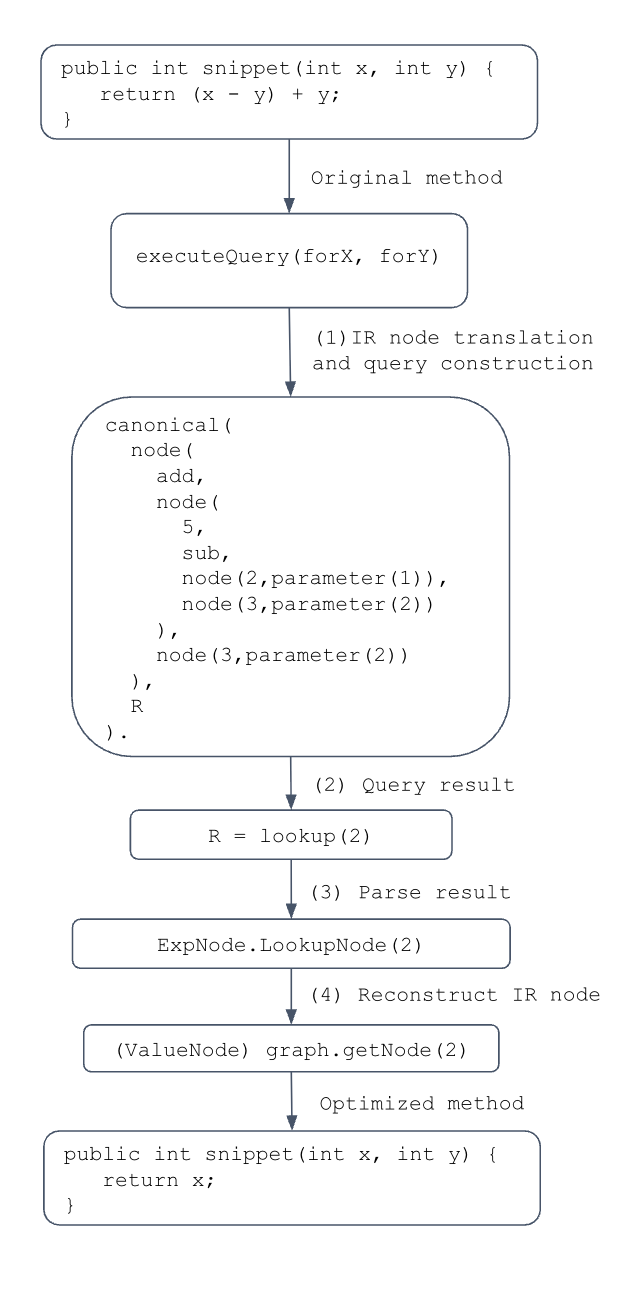
\includegraphics[width=0.5\textwidth]{./Packages/diagram.png}
    \caption{Prolog-Based Optimization Workflow}
    \label{fig:diagram}
\end{figure}
\renewcommand{\arraystretch}{1.3} % Increase row height
\setlength{\tabcolsep}{10pt}      % Optional: increase column separation

\chapter[Performance Evaluation]{Performance Evaluation}
This project defines an operation throughput metric to evaluate the impact of integrating Prolog into GraalVM. An operation is defined as the process of building the IR graph for a method and applying all optimization phases, including canonicalization, loop invariant reassociation, and conditional elimination. The operation is repeatedly performed for five seconds. The total number of completed operations is divided by five to calculate the average number of operations per second (operation throughput). This gives a consistent and stable throughput metric measured in operations per second, where a higher value indicates faster execution time. Benchmark is conducted twice: once using the standard GraalVM (without Prolog), and once after incorporating Prolog into GraalVM.
\subsection*{Canonicalization Tests}

Test Descriptions:
\begin{itemize}
    \item \textit{negateAdd}: $-y + x \rightarrow x - y$
    \item \textit{addNot}: $\sim x + x \rightarrow -1$
    \item \textit{addNeutral}: $0 + x \rightarrow x$
    \item \textit{addSubNode}: $(x - y) + y \rightarrow x$
\end{itemize}

Test Results:
\begin{table}[h]
    \centering
    \begin{tabular}{|l|r|r|r|}
        \hline
        $Test$ & $Without$ $Prolog$ & $With$ $Prolog$ & $Difference$ \\
        \hline
        $addNot$      & $2,964$ & $2,830$ & $-134$ \\
        $addSubNode$  & $3,050$ & $2,938$ & $-112$ \\
        $negateAdd$   & $2,242$ & $2,133$ & $-109$ \\
        $addNeutral$  & $3,005$ & $2,920$ & $-85$ \\
        \hline
    \end{tabular}
    \caption{Benchmark Results for Add Node Canonicalization Tests (Operations/Sec)}
    \label{table:Canonicalization}
\end{table}

\vspace{-10pt}

The benchmark results for the canonicalization tests (Table \ref{table:Canonicalization}) show minor performance reductions when using Prolog. The performance drop is minimal, with only slight decreases in operations per second. For example, in the \textit{negateAdd} test, throughput drops from 2,242 ops/sec to 2,133 ops/sec, and in the \textit{addNot} test, it decreases from 2,964 ops/sec to 2,830 ops/sec.
This slowdown is primarily attributed to the overhead introduced by the initial startup of the Prolog engine, which occurs for every optimization and is more pronounced in the case of stateful optimizations (conditional elimination).

\subsection*{Loop Invariant Reassociation Tests}
Test Descriptions:
\begin{itemize}
    \item \textit{subSub}: $(inv1 - i) - inv2 \rightarrow inv1 - inv2 - i$
    \item \textit{subAdd}: $(inv1 + i) - inv2 \rightarrow i + inv1 - inv2$
    \item \textit{addAdd}: $(inv1 + i) + inv2 \rightarrow i + inv1 + inv2$
    \item \textit{mulMul}: $(inv1 * i) * inv2 \rightarrow inv1 * inv2 * n$
\end{itemize}

Test Results:
\begin{table}[h]
    \centering
    \begin{tabular}{|l|r|r|r|}
        \hline
        $Test$ & $Without$ $Prolog$ & $With$ $Prolog$ & $Difference$ \\
        \hline
        $subAdd$ & $367$ & $330$ & $-37$ \\
        $subSub$ & $304$ & $268$ & $-36$ \\
        $addAdd$ & $375$ & $339$ & $-36$ \\
        $mulMul$ & $370$ & $334$ & $-36$ \\
        \hline
    \end{tabular}
    \caption{Benchmark Results for Reassociation Tests (Operations/Sec)}
    \label{table:Reassociation}
\end{table}

\vspace{-10pt}

Similarly, the reassociation tests (Table \ref{table:Reassociation}) reveal a modest slowdown when Prolog is used. Although there is some performance degradation, the effect of Prolog on the reassociation phase remains limited and does not severely impact throughput.

\subsection*{Conditional Elimination Tests}

Test Descriptions:
\begin{itemize}
    \item \textit{condElim1}: 2 nested ifs.
    \item \textit{condElim2}: An outer if containing 2 child if statements, one of which contains a nested if
    \item \textit{condElim3}: An outer if containing 3 child if statements, one of which contains a nested if.
    \item \textit{condElim4}: 8 nested ifs.
\end{itemize}

Test Results:
\begin{table}[h]
    \centering
    \begin{tabular}{|l|r|r|r|}
        \hline
        $Test$ & $Without$ $Prolog$ & $With$ $Prolog$ & $Difference$ \\
        \hline
        $condElim1$ & $1,661$ & $394$ & $-1267$ \\
        $condElim2$ & $1,386$ & $355$ & $-1031$ \\
        $condElim3$ & $951$ & $310$ & $-641$ \\
        $condElim4$ & $517$ & $243$ & $-274$ \\
        \hline
    \end{tabular}
    \caption{Benchmark Results for Condtional Eliminiation Tests (Operations/Sec)}
    \label{table:condElimination}
\end{table} 
\smallbreak

\vspace{-10pt}
The results in Table \ref{table:condElimination} show a noticeable drop in optimization throughput when Prolog is used for conditional elimination. The number of operations per second is significantly lower with Prolog across all tests. \textit{condElim1} is the simplest and fastest test as it only has 2 nested ifs, which is reflected in the much higher throughput without Prolog. However, when applying Prolog, its throughput drops the most, and all test results become more uniform. This is largely explained by Prolog’s significant startup overhead, which imposes a fixed cost that dominates the runtime for smaller tests. As a result, this overhead “levels” the performance across different test complexities, causing a uniform but overall slower throughput.

\chapter[Discussion]{Discussion}
This project successfully demonstrates the feasibility of integrating a Prolog engine into the GraalVM optimization pipeline using the Projog library. By translating GraalVM’s IR nodes into Prolog terms and implementing optimization logic as Prolog predicate rules, the system is able to perform a variety of compiler optimizations in a declarative and modular fashion. The results confirm that Prolog can be used as a backend for expressing compiler optimizations, making this integration both technically viable and functionally complete.

One key strength of the Prolog-based approach is its expressiveness. The declarative nature of Prolog allows optimization rules such as those for AddNode canonicalization to be written in a concise and readable manner that closely mirrors their mathematical definitions. This makes the logic easier to reason about and verify. However, during development, writing and debugging Prolog rules proved more challenging compared to Java. Prolog lacks the rich tooling and step-by-step debugging support available in Java environments, and its inference-based execution model can make it harder to trace errors or unexpected outcomes. Additionally, some optimization tasks, particularly conditional elimination, were difficult to express in a purely declarative form. This is partly due to the structure of the IR graph, which lacks direct parent-child relationships, necessitating dynamic fact assertions to capture control flow relationships during analysis.

Developing the Prolog representation format presented several challenges that required iterative refinement. A key difficulty was managing the initial incompatibility between the node representation and the evolving design of the Prolog rules used for analysis and optimization. The representation needed to balance simplicity with expressiveness; for example, deciding whether a control-flow node like \texttt{if} should include only the identifiers of its condition and successors, or also embed more detailed structural information, such as the full definitions of those subnodes. These decisions were guided primarily by experimentation. Similarly, designing the Prolog result parser involved several challenges. First, deciding on a clear and expressive grammar that could accurately capture the variety of IR node structures was critical. The grammar needed to be both precise and flexible to handle recursive nesting and different term types. Ensuring extensibility was another key challenge; as new IR node types and optimization patterns evolved, the parser had to accommodate these changes without significant rewrites. The use of the visitor pattern was instrumental in overcoming this, as it cleanly separates parsing from IR reconstruction logic and allows node-specific behavior to be encapsulated and extended independently. Throughout development, an iterative improvement approach was adopted. The Prolog representation format, parser grammar, logic, and visitor methods were refined based as more rules were introduced. This approach enabled incremental validation across components, ensuring the overall robustness and maintainability of the parser.

In terms of performance, the impact of Prolog integration varies depending on the nature of the optimization. Stateless rules like those used for canonicalization perform well, with only minimal overhead. This is achieved by using a singleton Projog instance that loads rules once and reuses them across invocations. On the other hand, stateful optimizations such as conditional elimination show significant slowdowns. These optimizations require reinitializing the Prolog engine for each run because of the need to assert and retract dynamic facts such as stamps to track known variable values. As a result, rule loading and engine setup must be repeated frequently, causing noticeable degradation. Furthermore, the Projog engine is relatively slow and could potentially be faster; however, due to time constraints, exploring other Prolog engine options was not possible.

Looking forward, several improvements could be explored. Investigating alternative Prolog engines or approaches might help reduce overhead. Finding ways to express conditional elimination rules in a purely declarative manner without requiring dynamic assertion of facts would simplify the integration and improve performance. Finally, it would be worthwhile to explore other optimization domains that are particularly well suited to declarative logic, where Prolog's strengths in pattern matching and symbolic reasoning can be leveraged more effectively.
\chapter[Conclusion]{Conclusions}
This project successfully demonstrated the feasibility of integrating Prolog-based optimization techniques into the GraalVM compiler framework. By converting GraalVM’s intermediate representation into Prolog terms and expressing optimizations as declarative rules, it was possible to implement a functional optimization pipeline within GraalVM using Projog. The results show that Prolog’s declarative syntax offers clear and expressive rule definitions, particularly well suited for stateless optimizations like canonicalization.

However, performance limitations were observed, especially for stateful optimizations such as conditional elimination. These phases suffered from significant overhead due to repeated engine initialization and dynamic fact management in Projog. While stateless optimizations incurred only minimal overhead thanks to reuse of a singleton Prolog instance, stateful optimizations were substantially slower. Additionally, the Projog engine itself proved relatively slow, and time constraints prevented exploring alternative Prolog implementations that might offer better performance.

Despite these challenges, the project highlights the potential of leveraging logic programming for compiler optimizations. The declarative nature of Prolog facilitates reasoning about optimization rules and modularizes the optimization logic. Future work could focus on identifying more performant Prolog engines, devising purely declarative methods for complex transformations like conditional elimination, and exploring other compiler optimization domains that can benefit from Prolog’s strengths in symbolic reasoning and pattern matching.



\bibliographystyle{IEEEtran}

\bibliography{./References/Bibliography}

\end{document}
